% !TeX root = ../thuthesis-example.tex

\chapter{引言}
\section{研究背景\label{sec:chap1-sec1}}
“物联网”这一术语通常指的是将网络的连接性和计算能力拓展到通常不被视为计算机的物体、传感器和日常物品,使这些设备能够在最小的人工干预下生成、交换和消费数据。物联网这一词汇最早由英国人 Kevin Ashton 在 1999 年用于描述一个系统,在该系统中,物理世界中的对象通过传感器连接到互联网\cite{li2015internet}。一些预测认为,到 2025 年,全球参与物联网的设备数可能达到 1000 亿台,对经济的影响超过 11 万亿美元\cite{rose2015internet}。

在 2013 年德国汉诺威工业展览会上,“工业 4.0”理念首度面世\cite{ghobakhloo2020industry},其中提及的工业物联网(Industrial Internet of Things, IIoT)在全球范围内引起了广泛关注。IIoT 关注将所有的工业资产,包括及其和控制系统,与信息系统和业务流程连接起来,从中收集的大量数据可以为工业生产、管理、解决方案设计提供重要的参考作用\cite{sisinni2018industrial}。工业物联网会产生大量工业数据,其类型包括时间序列、图片、视频、文档等,在某些场景下一年内甚至会产生 $4\times 10^{12}$ GB 数据\cite{ge2012riseofindustrial}。在这些数据中,时间序列数据主要由机器设备上的传感器采集产生,由于采集频率高、传感器数量多,成为了工业大数据的主体\cite{di2019industrial}。

工业物联网场景下的时序数据通常具有以下特点:
\begin{enumerate}
  \item 数据产生频率高。例如在风机发电场景下,国际风电标准 IEC 61400-25 规定,每台风机每秒需要采集 225 KB 数据,在某些极端工况下数据的采集频率需要提升至 8KHz\cite{李天安2020apache}。
  \item 数据总量大。长安汽车集团生产的每一辆汽车上均有数千个传感器,其车联网应用一共管理了近 12 亿条时间序列,每年产生的原始数据量超过 13,000 TB。
  \item 数据类型丰富。工业物联网场景下的时序数据除了由传感器产生的整形、长整形、单精度浮点数和双精度浮点数数据外,还可能包括由摄像头产生的图片、视频数据等。
\end{enumerate}

海量的时序数据对数据的写入、存储和查询都提出了挑战。传统的关系型数据库通常使用 B+ 树作为底层的存储数据结构,其在处理点写入、点查询等负载时具有较好的性能,但是在面对工业物联网场景下时序数据的高速率写入和聚合查询负载时性能较差,无法满足需求\cite{jensen2017time}。因此,一种专门为存储时序数据而设计的数据库应运而生,它们被称为时序数据库(Time Series Database,TSDB)。如图 \ref{fig:db-engine} 所示,在国际权威数据库流行度排行机构 DB-Engines 的调查结果中,时序数据库在过去十年内的流行度持续上升,目前其流行度仅次于图数据库,位居榜单中的第二名。

\begin{figure}
  \centering
  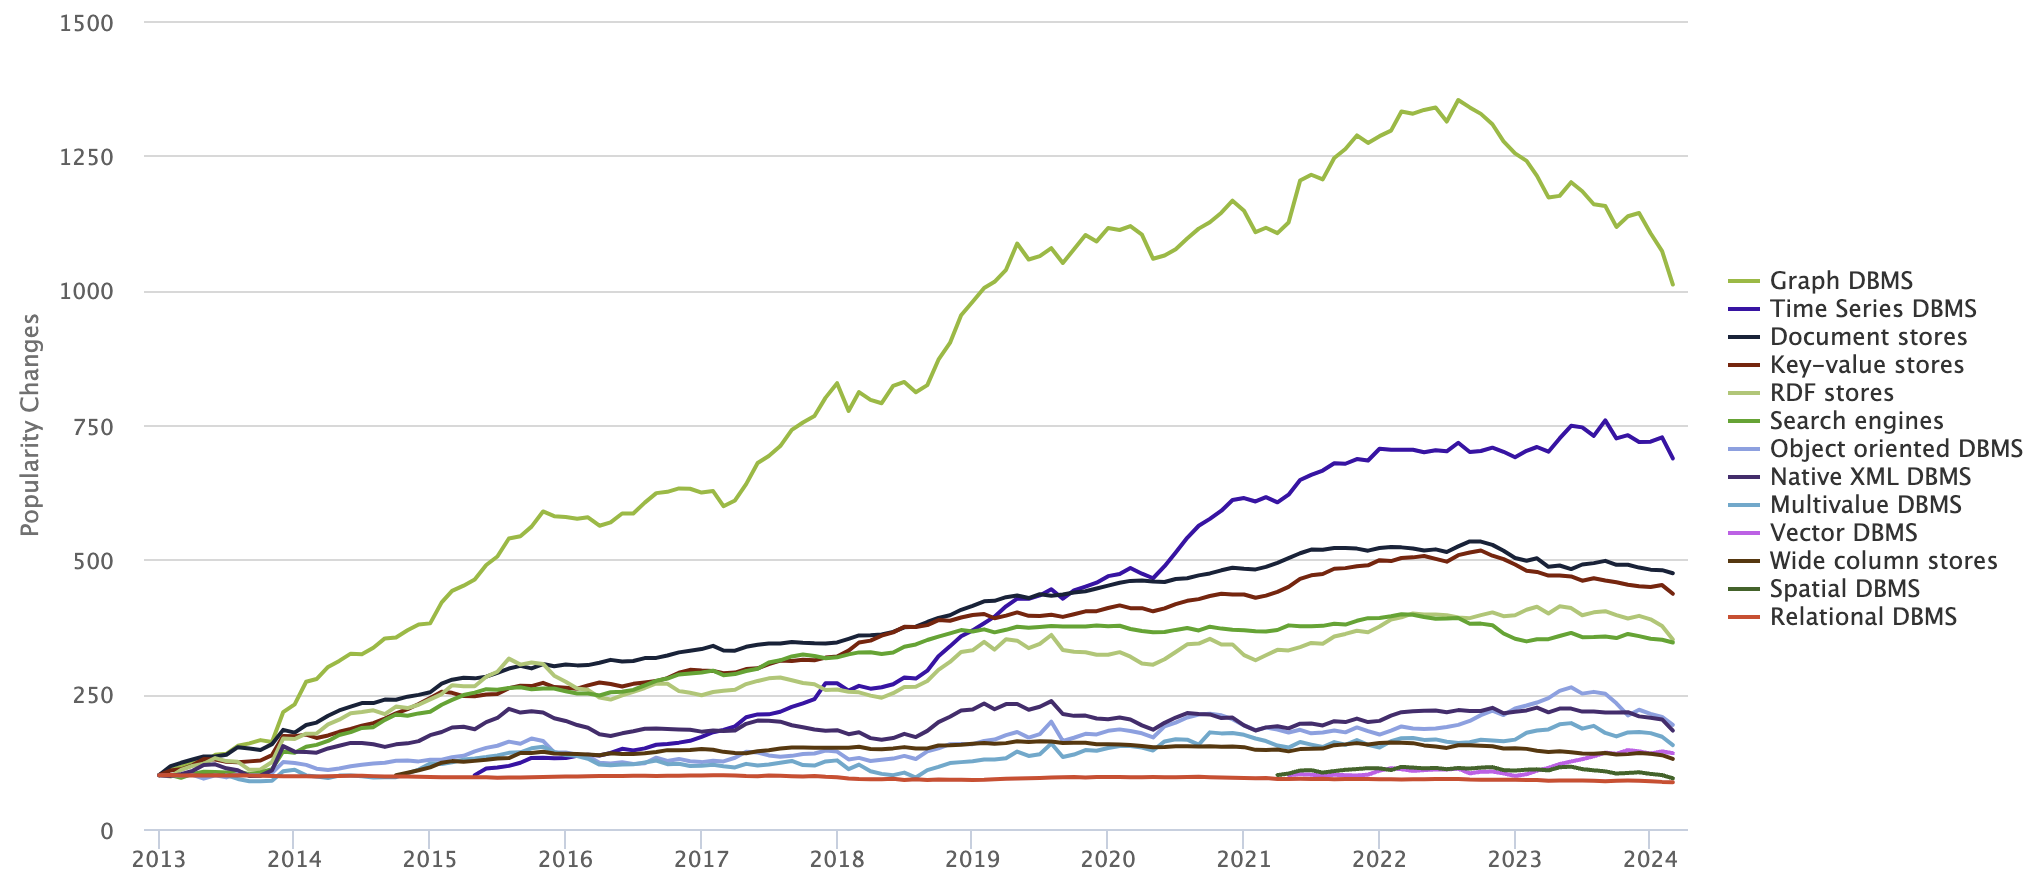
\includegraphics[width=\linewidth]{db-engines-ranking.png}
  \caption{DB-Engine 数据库类型流行度排名}
  \label{fig:db-engine}
\end{figure}

由于时序数据频率高、总量大、类型丰富的特点,时序数据库通常对数据的写入机制进行了针对性的优化,以满足工业物联网下时序数据高吞吐写入的需求。目前市面上流行的时序数据库主要有 Apache IoTDB\cite{wang2023apache}、InfluxDB\cite{naqvi2017time}、TDEngine\cite{tdengine2024github}、Apache HoraeDB\cite{apache2024horaedb} 等。其中 Apache IoTDB 是 Apache 基金会下一款开源的时序数据库,其具有为时间序列数据所优化的存储引擎、查询引擎以及分布式框架,可以满足工业物联网领域对海量时间序列数据高速写入、存储、快速读取以及复杂查询的需求\cite{wang2020apache}。

针对工业物联网场景下大量时序数据高速写入的需求,Apache IoTDB 主要提供了三种类型的数据写入接口:SQL 写入、按 Tablet 写入、按 Records 写入\cite{iotdb2024writedeletedata}。其中按 Records 写入是用户使用较为广泛的写入方式,但由于 IoTDB 目前按 Records 写入机制的设计和实现不佳,不仅在一般场景下会带来较大的写入开销,在序列数较多、数据量较大、并发量较高的场景下,这种写入方式也无法满足用户的写入需求。提升按 Records 写入的性能不仅能够满足极限场景下的用户需求,在普通场景下还可以减少服务器资源的占用,提高服务器的资源利用率,降低用户的使用成本,具有重要的现实意义和研究价值。因此,本文将重点研究为 Apache IoTDB 设计和实现一套高性能的按 Records 写入机制。
\section{Apache IoTDB 现有写入机制分析\label{sec:chap1-sec2}}
\subsection{Apache IoTDB 现有写入接口介绍}
如前文所述,目前 Apache IoTDB 提供了三种写入接口:使用 SQL 写入、按 Tablet 写入(\emph{InsertTablets})、按 Records 写入(\emph{InsertRecords})。表 \ref{tab:iotdbwriteinterfacecompare} 对这三种写入接口进行了对比。

SQL 写入指的是使用形如 \emph{insert into root.sg.d1(timestamp, s1, s2) values(1, 1, 2)} 的 SQL 语句进行写入。客户端将写入 SQL 发送到服务器,服务器对 SQL 进行解析并生成写入请求,然后将写入请求交由存储引擎处理。这种写入方式较为灵活,也是大部分数据库都会提供的一种写入方式。但是,由于每次写入时都需要进行 SQL 的解析,这一部分开销不可忽视,因此这种方式的写入性能较差。在生产场景中,几乎没有用户使用这种写入方式。

按 Tablet 写入和按 Records 写入是 Apache IoTDB 提供的一种原生写入接口,用户将写入请求直接以数据结构的形式传递给客户端,然后客户端通过 RPC 层将这些参数传输到服务器端,服务端可以直接从 RPC 层得到写入请求,而无需进行 SQL 解析等流程。因此,这两种写入接口的性能远优于通过 SQL 写入的性能。

在 Apache IoTDB 中,一条或多条时间序列归属于同一个设备(Device)\cite{apache2024iotdbdevice}。一个设备对应了现实世界中的一个实体,是一个在现实世界中拥有若干个物理量的设备或装置,例如一台风力发电机、一辆汽车、一台计算机等。每个设备在 IoTDB 中都有唯一的 ID,称为设备 ID。每个设备下的时间序列也有其 ID,称为时间序列 ID。每条时间序列都可以用设备 ID 和时间序列 ID 作为其唯一标志符。

按 Tablet 写入就是将一批数据组织成名为 Tablet 的数据结构发送到服务器端。一个 Tablet 是一个设备在一段时间内的多行数据,每一行数据都有不同的时间戳。按 Tablet 写入其实是在时间维度上将同一个设备的数据聚集起来批量写入,不同设备的数据则无法聚集在同一个 Tablet 中。批量写入的好处是可以将写入流程中的某些固定开销(例如元数据校验、执行流程中的锁获取等)均摊到一批数据上,进而提升写入的性能。因此,如果想要获得较好的性能,单个 Tablet 的大小不能过小,不然就失去了批量化写入的优势。

按 Tablet 写入的方式非常适合单设备数据高频产生的场景,因为数据产生的频率很快,在较短时间内就可以积攒起一个 Tablet 进行写入,数据从产生到能够被查询到的延迟较低。但是在单设备数据低频产生的场景下,如果按 Tablet 进行写入,则需要较长时间才能积攒出一个合适大小的 Tablet,数据从产生到能够被查询到的延迟会大大增加。例如在长安汽车的车联网场景中,一辆汽车就是建模时的一个设备,汽车中的每个传感器(如胎压、水温等)则是设备下的时间序列,每辆汽车每 30 秒采集一次车内传感器的数据,如果按照一个 Tablet 有 100 行数据计算,那么每辆汽车的数据从产生到能够被查询到的延迟会达到 50 分钟,这是无法接受的。

按 Records 写入是数据批量化写入的另一种形式。一条 Record 是一个设备在一个时间戳下产生的数据,Records 就是多个 Record 的组合,可能包含多个设备在多个时间戳下记录的数据。这种写入方式其实是在时间和设备两个维度上将数据聚集在一起进行批量写入。因此,这种写入方式避免了按 Tablet 写入的缺点,即使单个设备产生数据的频率非常低,也可以将其数据聚集在一起进行批量写入,既通过批量化写入提升了写入性能,又避免了数据从产生到能够被查询到的延迟过大的问题。因此,按 Records 写入是目前 Apache IoTDB 中适用场景最广的写入方式。但是,由于过去设计和实现的原因,在单设备数据高频写入等场景下按 Records 写入的性能与按 Tablet 写入有一定差距,因此如何优化按 Records 写入的设计和实现进而提升其性能是本文关注的重点。

\begin{table}
  \centering
  \caption{Apache IoTDB 写入接口对比}
  \begin{tabular}{lp{3.5cm}p{3.5cm}p{3.5cm}}
    \toprule
    写入接口  & 优点 & 缺点 & 适用场景 \\
    \midrule
    SQL 写入 & 灵活 & 性能较差 & 用户测试或少量数据写入 \\
    按 Tablet 写入  & 性能最好,可以将写入流程中的某些固定开销均摊到一批数据上 & 单设备数据低频产生的场景下,数据从产生到真正写入的延迟较大 & 单设备数据高频产生的场景\\
    按 Records 写入  & 性能较好,即可以通过批量化写入获取不错的性能,又降低了数据从产生到真正写入的延迟 & 由于设计和实现原因,性能与按 Tablet 写入有差距 & 单设备数据低频产生的场景 \\
    \bottomrule
  \end{tabular}
  \label{tab:iotdbwriteinterfacecompare}
\end{table}

\subsection{Apache IoTDB 现有按 Records 写入机制实现}
如图\ref{fig:iotdb-write-process}所示,目前 Apache IoTDB 按 Records 写入流程主要分为三个阶段:
\begin{enumerate}
  \item \textbf{客户端侧数据预处理}。此阶段从客户端的行式写入函数被用户调用开始,到客户端调用远程过程调用层的数据发送方法前结束。这个阶段进行的工作是校验用户传入的参数是否合法,检验客户端状态,选取合适的服务器节点作为数据发送的目标(在分布式部署时可能存在多个服务器节点),对数据进行部分序列化。
  \item \textbf{远程过程调用层数据传输}。远程过程调用(Remote Procedure Call,RPC)层跨越了客户端侧和服务器侧,其负责的主要工作为:将客户端侧传入的数据根据预定义的结构序列化为二进制的数据流,并通过网络传输到服务器侧,再反序列化为预定义的数据结构,交由服务器中 IoTDB 上层的处理逻辑完成后续流程。
  \item \textbf{IoTDB 处理写入请求}。此时写入请求被 RPC 层反序列化为预定义的写入请求数据结构,IoTDB 会进行时间序列 ID 和路径校验、元数据校验、权限校验、MPP 框架处理、内存控制处理、监控框架记录性能指标、写预写日志(Write Ahead Log,WAL)、写入内存表、更新内存索引等步骤,将数据记录在内存和磁盘中。这一步结束以后,整个写入请求就被成功执行了。
\end{enumerate}
\begin{figure}
  \centering
  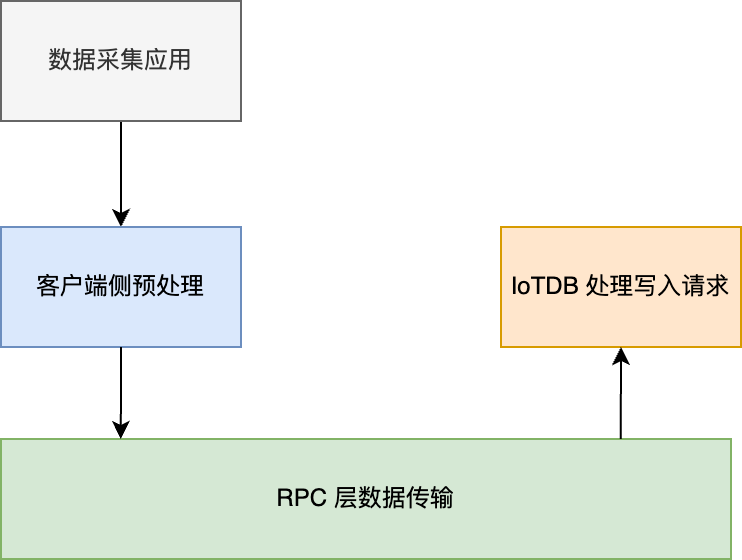
\includegraphics[width=0.7\linewidth]{数据写入整体过程.png}
  \caption{Apache IoTDB 行式写入流程}
  \label{fig:iotdb-write-process}
\end{figure}
\subsection{Apache IoTDB 现有行式写入机制不足}
经过在某些用户场景和压力测试场景下对 Apache IoTDB 的按 Records 写入机制的测试和分析,本文发现目前的实现有以下问题:
\begin{enumerate}
  \item \textbf{服务器侧写入逻辑的实现不够高效}。当一批记录一起到达 IoTDB 的服务端后,目前的实现仍然是逐条进行写入,而不是批量化地写入。这样的实现方式需要对每一行记录都获取写入路径上的多个锁,在监控框架中更新指标,调用很多预处理和后处理函数,这些操作都会带来很大的开销,使得服务器上真正用于记录数据的时间变得很少,资源利用比较低效。
  \item \textbf{RPC 层设计不够合理}。目前 IoTDB 所使用的 RPC 框架是 Apache Thrift,然而目前行式写入接口的实现几乎直接将客户端传入的参数放到了 Thrift 中进行传输。这并没有利用好传入数据的特点,例如不同记录的时间戳范围都比较接近,设备和时间序列 ID 具有一定的相似性。利用这些特点可以对传输的数据进行压缩,减少传输的数据量,提高传输的效率。
  \item \textbf{对客户端侧的资源利用不足}。目前 IoTDB 的客户端侧所执行的工作较为轻量,而将部分与上下文无关的工作,如路径语法校验、内存占用计算等工作留到了服务器侧,这并没有充分利用客户端侧的资源,也没有充分利用客户端侧的计算能力。
\end{enumerate}
由于篇幅原因,对原有行式写入机制不足的详细分析将在后续章节中进一步展开。
\section{研究内容}
结合 \ref{sec:chap1-sec1} 和 \ref{sec:chap1-sec2} 节的分析,本文发现目前 Apache IoTDB 的行式写入接口具有较好的灵活度,但是过去的实现机制在性能上存在一定的不足,在时间序列数较多、写入数据量较大的场景下无法很好地满足用户需求。因此,本工作的研究内容主要包括:
\begin{enumerate}
  \item 如何寻找目前 Apache IoTDB 的不足。目前 IoTDB 的行式写入性能与列式写入性能大约有 2-3 倍的差距,分析这个差距产生的原因并找出目前行式写入机制的设计缺陷和实现缺陷有助于我们在设计新的行式写入机制时避免这些问题。
  \item 如何在保持对原有行式写入接口兼容的情况下设计并实现一套高性能的行式写入机制。由于目前使用 Apache IoTDB 行式写入接口的用户众多,因此在设计新的行式写入机制时需要保持对原有接口的兼容,以减少用户迁移的成本。同时,新的行式写入机制需要从客户端、RPC 层、存储引擎等多个方面进行优化,以提高行式写入的性能。
  \item 如何对 Apache IoTDB 的行式写入机制进行性能评估与分析。设计并实现一套高性能的行式写入机制后,需要对其进行性能评估与分析,以验证其性能的提升效果。目前的性能测试工具并不能很好地反映用户的真实写入场景,因此需要开发一套模拟用户场景的测试工具,收集一些真实用户场景的写入特征,并使用测试工具根据这些特征模拟不同用户的写入场景,验证并分析 Apache IoTDB 行式写入机制的性能。
\end{enumerate}

\section{研究贡献}
本文的主要贡献体现在以下三个方面:
\begin{enumerate}
  \item \textbf{对目前 Apache IoTDB 已有行式写入机制的性能分析}。本工作对目前 Apache IoTDB 的已有行式写入机制进行性能分析,包括对其性能的评估、寻找其性能瓶颈、分析其设计不足等。
  \item \textbf{为 Apache IoTDB 设计并实现一套高性能的行式写入机制}。本工作在吸收目前行式写入机制的优点的基础上,分别对客户端、RPC 层、存储引擎侧进行优化,设计并实现一套高性能的行式写入处理机制,以提高 IoTDB 的行式写入性能。
  \item \textbf{对 Apache IoTDB 的行式写入机制进行性能评估与分析}。本工作开发了一套模拟用户场景的测试工具,收集了一些真实用户场景的写入特征,并使用测试工具根据这些特征模拟不同用户的写入场景,验证并分析 Apache IoTDB 行式写入机制的性能。
\end{enumerate}

\section{本文的组织结构}

本文一共分为九章,每个章节的内容如下:

第 1 章为引言部分,主要介绍了物联网和工业物联网发展背景下时序数据库发展的意义,并介绍了目前 Apache IoTDB 的三种写入方式及其优缺点和适用场景,并阐述了目前 Apache IoTDB 按 Records 写入的不足之处,最后引出了本工作的研究内容和贡献。

第 2 章介绍了相关工作,首先介绍了主流时序数据库的写入接口和实现,然后介绍了主流时序数据库的存储引擎设计,最后介绍了数据库客户端与 RPC 相关的优化工作。

第 3 章详细介绍了目前 Apache IoTDB 的行式写入机制的运行流程,包括客户端侧的数据预处理、RPC 层的数据传输、IoTDB 服务端的写入处理等,并通过 Arthas 等性能分析工具对这一机制的性能进行了分析,找出了其性能瓶颈,并指出其在设计上和实现上的不足之处。随后从整体上介绍了本工作的设计目标和设计思路,包括对客户端、RPC 层、存储引擎的设计思路,以及设计新的行式写入机制的一些原则和约束,为读者对本工作提供一个整体的认识。

第 5 章介绍了对客户端侧的设计和实现,包括对客户端侧的数据预处理、行式写入转列式写入、路径校验、内存开销预计算等方面的设计与实现,并介绍了实现过程中的一些细节。

第 6 章介绍了对 RPC 层的设计和实现,介绍了行式序列化和列式序列化两种 RPC 包设计方案,讨论了这两种方案的优劣,并说明了最终选择列式序列化的原因,最后介绍了 RPC 层的实现细节。

第 7 章介绍了存储引擎侧高性能行式写入机制的设计与实现,包括批量化写入、计划片级并行写入、预写日志优化等。

第 8 章是实验部分,首先介绍了用于模拟用户场景的测试程序的设计,然后介绍了包括中冶赛迪、长安汽车、四维智联等用户的典型写入场景,最后使用模拟测试工具和 IoT-Benchmark\cite{liu2019benchmarking} 两种测试工具对新的行式写入机制进行了性能测试,并对测试结果进行了分析。

第 9 章是总结部分,总结了本文的工作,指出了本文的不足之处,并对未来的工作进行了展望。